\noindent
\begin{minipage}[t]{0.25\textwidth}
    % Cột lề trái: dóng Hình 10 đúng ngang hàng với Box 6 và đoạn giải thích bên dưới
    \vspace*{10.2cm}
    \centering
    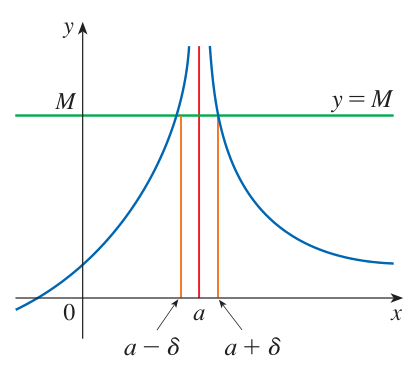
\includegraphics[width=\linewidth]{images/p0147_fig1.png}
    
    \vspace{4pt}
    \raggedright
    {\small\textbf{\textsf{HÌNH 10}}}
\end{minipage}%
\hfill
\begin{minipage}[t]{0.72\textwidth}
    % Cột nội dung chính
    Đặt $\delta = \min\{\delta_1, \delta_2\}$, là số nhỏ hơn trong hai số $\delta_1$ và $\delta_2$. Chú ý rằng
    \[
    \begin{aligned}
    &\text{nếu}\qquad 0 < |x - a| < \delta \qquad \text{thì}\qquad 0 < |x - a| < \delta_1 \qquad \text{và}\qquad 0 < |x - a| < \delta_2 \\[3pt]
    &\text{và do đó}\qquad |f(x) - L| < \frac{\varepsilon}{2} \qquad\text{và}\qquad |g(x) - M| < \frac{\varepsilon}{2}
    \end{aligned}
    \]
    Do đó, theo (5),
    \begin{align*}
    |f(x) + g(x) - (L + M)| &\leqslant |f(x) - L| + |g(x) - M| \\[2pt]
    &< \frac{\varepsilon}{2} + \frac{\varepsilon}{2} = \varepsilon
    \end{align*}
    Tóm lại,
    \[
    \text{nếu}\qquad 0 < |x - a| < \delta \qquad \text{thì}\qquad |f(x) + g(x) - (L + M)| < \varepsilon
    \]
    Như vậy, theo định nghĩa của giới hạn,
    \[
    \lim_{x \to a} [f(x) + g(x)] = L + M \tag*{$\textcolor{stewartred}{\blacksquare}$}
    \]

    \vspace{0.8em}
    \noindent{\color{stewartcyan}\rule{1.1ex}{1.1ex}}\quad \textbf{\large\textsf{Giới hạn vô cực}}

    \vspace{0.2em}
    Các giới hạn vô cực cũng có thể được định nghĩa một cách chính xác. Dưới đây là phiên bản chính xác của Định nghĩa 2.2.4.

    \begin{definitionbox}
        \noindent\tcbox[
            colback=white,
            colframe=stewartred,
            boxrule=0.8pt,
            arc=1.5pt,
            top=1.5pt, bottom=1.5pt, left=3.5pt, right=3.5pt,
            on line
        ]{\textbf{\color{stewartred}\textsf{6}}}\;
        \textbf{\textsf{\color{stewartred}Định nghĩa chính xác của giới hạn vô cực}}\quad
        Giả sử $f$ là một hàm số xác định trên một khoảng mở nào đó chứa số $a$, có thể ngoại trừ tại chính $a$. Khi đó
        \[
        \lim_{x \to a} f(x) = \infty
        \]
        có nghĩa là với mọi số dương $M$, tồn tại một số dương $\delta$ sao cho
        \[
        \text{nếu}\qquad 0 < |x - a| < \delta \qquad\text{thì}\qquad f(x) > M
        \]
    \end{definitionbox}

    Điều này nói lên rằng các giá trị của $f(x)$ có thể lớn tùy ý (lớn hơn bất kỳ số $M$ cho trước nào) bằng cách yêu cầu $x$ đủ gần $a$ (trong khoảng cách $\delta$, trong đó $\delta$ phụ thuộc vào $M$, nhưng với $x \neq a$). Một minh họa hình học được cho trong Hình 10.

    Cho bất kỳ đường nằm ngang nào $y = M$, ta có thể tìm được một số $\delta > 0$ sao cho nếu ta giới hạn $x$ nằm trong khoảng $(a - \delta, a + \delta)$ với $x \neq a$, thì đường cong $y = f(x)$ sẽ nằm phía trên đường thẳng $y = M$. Bạn có thể thấy rằng nếu một giá trị $M$ lớn hơn được chọn, thì có thể cần một $\delta$ nhỏ hơn.

    \vspace{0.8em}
    \noindent\textbf{\textsf{\color{stewartcyan}VÍ DỤ 5}}\quad Sử dụng Định nghĩa 6 để chứng minh rằng $\displaystyle\lim_{x \to 0} \frac{1}{x^2} = \infty$.

    \vspace{0.3em}
    \noindent\textbf{\textsf{\color{stewartcyan}LỜI GIẢI}}\quad Cho $M$ là một số dương cho trước. Ta muốn tìm một số $\delta$ sao cho
    \[
    \text{nếu}\qquad 0 < |x| < \delta \qquad\text{thì}\qquad 1/x^2 > M
    \]
    \[
    \text{Nhưng}\qquad \frac{1}{x^2} > M \quad\iff\quad x^2 < \frac{1}{M} \quad\iff\quad \sqrt{x^2} < \sqrt{\frac{1}{M}} \quad\iff\quad |x| < \frac{1}{\sqrt{M}}
    \]
    Vì vậy nếu ta chọn $\delta = 1/\sqrt{M}$ và $0 < |x| < \delta = 1/\sqrt{M}$, thì $1/x^2 > M$. Điều này chứng tỏ rằng $1/x^2 \to \infty$ khi $x \to 0$. \hfill {\color{stewartcyan}$\blacksquare$}
\end{minipage}

\vfill
\begin{center}
    \fontsize{6.5}{8}\selectfont \color{stewartgray}
    Copyright 2021 Cengage Learning. All Rights Reserved. May not be copied, scanned, or duplicated, in whole or in part. WCN 02-200-203\\
    Due to electronic rights, some third party content may be suppressed from the eBook and/or eChapter(s). Editorial review has deemed that any suppressed content does not materially affect the overall learning experience. Cengage Learning reserves the right to remove additional content at any time if subsequent rights restrictions require it.
\end{center}
